%\documentclass[aps,prl,twocolumn,nobibnotes]{revtex4}
\documentclass[aps,showpacs,twocolumn,nobibnotes]{revtex4}
%\documentclass[aps,preprint,showpacs,nobibnotes]{revtex4}
%\documentclass[aps,preprint,nobibnotes]{revtex}
\usepackage{graphics,graphicx,amsfonts,amsmath,amsbsy,amssymb,color}
\usepackage{bm}
%\usepackage{epic}
%\usepackage{mciteplus}
\usepackage{subfigure}
\usepackage{vector}  % Allows "\bvec{}" and "\buvec{}" for "blackboard" style bold vectors in maths
\newcommand{\D}[1] {D_{\bf #1}}
\def \beq {\begin{eqnarray}}
\def \eeq {\end{eqnarray}}
\def \Schrodinger {{Schr\"{o}dinger }}
\def \Di {{D_{\bfi}}}
\def \Dj {{D_{\bfj}}}
\newcommand {\adag}[1] {{a_{#1}^\dagger}}
\def \bfj {{\bf j}}
\def \bfi {{\bf i}}
\def \rone {{\bvec{r}_1}}
\def \rtwo {{\bvec{r}_2}}
\def \mEh {{\textrm{mE}_{\textrm{h}}}}
\def \Eh {{\textrm{E}_{\textrm{h}}}}
\def \nadd {{n_a}}
\newcommand{\braket}[3] {{\langle #1 | #2 | #3 \rangle}}
\newcommand{\brket}[2] {{\langle #1 | #2 \rangle}}
\newcommand{\bra}{\ensuremath{\langle}}
\newcommand{\ket}{\ensuremath{\rangle}}
%\def \ham {{\bf H}}
\def \ham {{\hat{H}}}
%\def \Sz {{\hat{\textrm{S}_{\textrm{z}}}}}
\def \Sz {{\hat{S}_z}}
\newcommand{\rff}[1]{{Eq.~\eqref{#1}}}
\def \Pgen {{P_{\textrm{gen}}}}
\def \Carb {{\textrm{C}_{\textrm{2}}}}
\def \Hij {{H_{\bvec{i}\bvec{j}}}}
\def \Kii {{K_{\bvec{i}\bvec{i}}}}
\def \Kij {{K_{\bvec{i}\bvec{j}}}}

\begin{document}
\title{Spectral functions of extended systems via quantum embedding}
\author{George~H.~Booth}
%\email{ghb24@cam.ac.uk}
\author{Garnet~Kin-Lic~Chan}  
\affiliation{Department of Chemistry, Frick Laboratory, Princeton University, Princeton, New Jersey 08544, USA}

\begin{abstract}
The density matrix embedding theory (DMET) was introduced recently, and displayed the ability to seamless embed strongly entangled ground-state wavefunctions
within an extended environment [PRL {\bf 109} 186404 (2012)].
%With similarities 
%to the dynamical mean-field method, a set of local sites are self-consistently correlated, but with an analytically constructable bath describing the
%coupling to the rest of the extended system. 
Despite many formal advantages in the analytic embedding, the method was restricted to static, ground-state properties.
Here, we generalize the concept of quantum embedding to introduce a frequency dependence and demonstrate accurate spectral functions at a tiny
computational cost. Through this quantum embedding of a local spectral function within a mean-field response over the whole system, 
a coupling of the delocalized excitations is captured through a small set of 
analytically constructed, and now frequency-dependent bath states. In contrast to dynamical mean-field theory, the resultant 
spectral functions are directly obtained on the real-frequency axis, with no bath discretization error, and allow for straightforward generalization both 
to impurity clusters and arbitrary electron perturbation operators. We demonstrate
the application of this method to the Hubbard model, where we believe that for the low-energy excitations, these results represent some of the most accurate 
zero temperature, thermodynamic limit spectral functions for the Hubbard model to date, and demonstrate the trivial extension to two-particle Greens functions. 
This vastly extends the scope and applicability 
of the DMET method in condensed matter problems as a computationally tractible route to correlated spectral functions of extended systems.
\end{abstract}
\date{\today}
\maketitle

Dynamic correlation functions are directly probed in most spectroscopic methods, as well as other techniques such as scanning tunnelling microscopy (STM), 
and correspond to many of the important transport, optical, magnetic and wider electronic structure properties of materials. 
As such, their accurate computational prediction is highly sought after within the materials science community. 
However, few robust approaches exist for strongly correlated problems\cite{Gali2013}. The difficulty is in simultaneously requiring both an accurate 
treatment of the electron correlations beyond mean-field band theory for the ground state {\em and} excitation spectrum, as well as modelling 
a system of sufficient size to mimic the thermodynamic limit of bulk properties and not suffer spurious finite size effects. 
However in general, it is only mean-field electronic structure methods which are computationally cheap enough to access the required system
sizes, and so there is a pressing need for methods with mean-field scaling, which can account for the excitation spectrum in strongly correlated 
and entangled systems.

A general, zero-temperature dynamic correlation function can be defined in the frequency domain as
\begin{equation}
    G(\omega;A,V) = \langle \Psi_0 | A^{\dagger} \frac{1}{\omega-(H-E_0)+i \eta} V | \Psi_0 \rangle , \label{eqn:intCorrFunc}
\end{equation}
with the one- and two-particle Greens functions defined with $V$ and $A$ being single annihilation/creation operators or neutral excitation
operators respectively, with appropriate time-ordering of the operators. Spectral quantities are then defined as $A(\omega)=-\frac{1}{\pi}\Im[G(\omega)]$,
where the spectral broadening is given by the small imaginary component of the energy, $\eta$, which regularizes the correlation function. The single particle
density of states is given by the spectral representation of the one-particle Greens function, experimentally measured within STM 
and (angle-resolved) photoemission spectroscopy. However, other spectral functions are also highly sought after, such as the two-hole propagator, 
probed with Auger spectroscopy\cite{Mona2013}, or the two-electron Greens function, a key descriptor in Raman spectroscopy, and in the 
mechanism of high-$T_c$ superconductivity\cite{Millis2012,Millis2013}.

One such method which has proven successful in obtaining strongly correlated spectral functions is dynamical mean-field theory (DMFT). In 
DMFT, the central variable is the local, one-particle Greens function, which is self-consistently embedded within a non-interacting or 
mean-field Greens function over the system. This is mapped to an impurity problem, which is then solved via an `impurity solver', such as 
continuous-time quantum Monte Carlo (CT-QMC). However, there are some formal drawbacks of the DMFT formulation. If CT-QMC is used as an 
impurity solver (or indeed general QMC methods used in isolation), then the spectral functions are obtained only on the imaginary frequency 
axis, requiring unstable analytic continuation onto the real frequency axis, which can wash out the subtle or sharp features of the 
spectra\cite{Thomas2011}. Alternative solvers such as exact diagonalization suffer from bath discretization error in the spectra due to the 
representation of the continuous Weiss field (at all frequencies) by a finite number of bath sites. In addition, since DMFT
is formulated from the one-particle Greens function, alternative spectra such as the two-particle Greens function and optical spectra are 
not straightforward to obtain, formally requiring expensive vertex corrections to compute\cite{Millis2012}. Other methods to calculate 
spectra of correlated extended systems, such as the dynamical density matrix renormalization group\cite{Jeckelmann2004} or cluster perturbation 
theory\cite{Senechal2000} are restricted to certain correlation strengths or spatial dimensions.

Here, we aim to circumvent these issues, by generalizing and extending the idea of quantum embedding of {\emph states}, as introduced in 
Ref.~\onlinecite{Chan2012}. This is achieved by embedding a local correlation function defined over a set of `impurity' sites, within an 
analytic coupling to the rest of the delocalized excitation space. This is determined through the Schmidt decomposition of a mean-field 
response computed throughout the bulk system. This renders exact limits of the spectra in the non-interacting and local excitation limits. 
Since the method is formulated in terms of a general response vector, it is also not restricted in the type or rank of perturbation 
operators that it can consider. Furthermore, since the analytic coupling is only defined for a given frequency (rather than all frequencies 
for DMFT), the entanglement bath for the spectra is compact and exactly represents the coupling defined by the global response function. This 
allows for large impurity clusters to be treated with small numbers of additional `bath' states, without discretization error in the coupling 
to the extended system, and direct evaluation of spectra on the real frequency axis. The approach will be demonstrated for the Hubbard model, 
defined by the Hamiltonian in the site basis as
\begin{equation}
    H = -t \sum_{\langle ij \rangle, \sigma} a_{i,\sigma}^{\dagger}a_{j,\sigma} + U \sum_i n_{i,\uparrow} n_{i,\downarrow} - \frac{U}{2}\sum_i (n_{i,\uparrow} + n_{i,\downarrow})  . \label{eqn:hub}
\end{equation}
This lattice model encapsulates many of the difficulties in the electronic structure of correlated materials, displaying correlation driven 
phase transitions in the thermodynamic limit, and is closely representative of many transition metal oxides, including qualitative aspects 
of high-$T_c$ superconductivity\cite{Millis2013,Anderson87}. Where possible, we compare to one-dimensional exact results\cite{Lieb68,Ovchinni1970}, as 
well as large-scale DMFT calculations\cite{Go2009}, also demonstrating spectra for the doped system and two-particle Greens functions.

\emph{Method.-} Within the analytic quantum embedding formalism introduced for the ground state with the DMET method (see 
Ref.~\onlinecite{Chan2012,Chan2013} for details), the coupling between the correlated `impurity' sites, $\{ |\alpha \rangle \}$, and the rest 
of the system is represented via the component of the Schmidt basis of a single Slater determinant which couples the impurity space to 
the `environment' space external to the impurity. This analytic coupling is represented by a one-electron space of the same dimension as 
the impurity size, and denoted the ground-state {\em bath}, $\{ |\beta \rangle \}$. This space then spans the exact entanglement of the 
impurity space to its environment, as defined by the original mean-field function over the entire extended lattice. The interacting Hamiltonian 
is then projected into this space, which is now independent of the total number of sites in the system, and solved to return a ground-state 
wavefunction, $|\Psi_0 \rangle$, in the space of $\{ |\alpha \rangle \} \otimes \{ |\beta \rangle \} \otimes \rm{det[ext]}$, where det[ext] 
represents the space of one-electron functions which are uncoupled to the impurity cluster after the Schmidt decomposition. Along with the 
bath space, a self-consistency procedure returns a one-electron interaction potential, $u$ which describes some of the longer-ranged 
correlation effects, and controls the effective number of electrons in the impurity cluster.

We now generalize this procedure for embedding within a linear response vector determined from a one-electron Hamiltonian, $h$, which spans the 
entire lattice, in order to create a set of now frequency-dependent bath states into which the interacting problem can be projected. 
The global response across the lattice is constructed as,
\begin{equation}
|\phi^{(1)}(\omega) \rangle = \left[ \omega-(h-\varepsilon_0)+i\eta \right]^{-1} {\hat V} |\phi^{(0)}\rangle = 
    {\hat G_0}(\omega) {\hat V} |\phi^{(0)} \rangle  , \label{nonintGF}
\end{equation}
where $h = t + u$ is a static, one-electron Hamiltonian over the lattice, defined by the non-interacting part of the Hamiltonian 
in Eq.~\ref{eqn:hub}, and the interaction potential obtained from the ground-state self-consistency condition over the impurity space. 
For simplicity, we restrict ourselves in this letter to the case of {\em local} spectral functions, where $V$ and $A$ both act solely 
in the impurity space, although extensions to non-local perturbations will be detailed in a forthcoming paper. This means that the operator 
${\hat V}$, as well as $|\phi^{(0)} \rangle$, the ground-state mean-field determinant, are both spanned by the original ground-state DMET 
space of $\{ |\alpha \rangle \} \otimes \{ |\beta \rangle \} \otimes \rm{det[ext]}$. The frequency-dependent coupling to the environment 
results from the ${\hat G_0}$ operator, and we now Schmidt decompose its action onto ${\hat V} |\phi^{(0)} \rangle$, in order to isolate 
the coupling at each frequency point between the environment and fully correlated space of impurity sites and ground-state bath (i.e. 
$\{|\alpha \rangle \} \oplus \{|\beta \rangle \} \equiv \{ \gamma \rangle \}$). The space external to this to which the coupling is defined 
is denoted by $n$. We choose to partition the response into these spaces to ensure that at all frequencies, we span the correlated ground-state 
DMET wavefunction, $|\Psi_0 \rangle$.

The action of ${\hat G_0}(\omega){\hat V}$ on $|\phi^{(0)} \rangle$ can be easily found in the eigenbasis of $h$, $\{ |\chi_r \rangle ; \epsilon_r \}$, 
and rotated such that the operators act solely within the partitioned spaces. For instance, with ${\hat V}=a_{\alpha}$, 
\begin{equation}
    {\hat G_0}(\omega){\hat V} = \sum_{\gamma} X_{\gamma}(\omega) a_{\gamma} + \sum_{n} X_{n}(\omega) a_n  ,
\end{equation}
with
\begin{equation}
    X_n(\omega) = \sum_{r \in {\mathrm occ}} \frac{|n \rangle \langle n|\chi_r \rangle \langle \chi_r | a_{\alpha} | \phi^{(0)} \rangle}{\omega - \epsilon_r + i \eta}   .
\end{equation}
For a two-index perturbation such as ${\hat V}=a_{\alpha}^{\dagger}a_{\alpha}$, the operator can be similarly decomposed as,
\begin{equation}
    {\hat G_0}(\omega){\hat V} = \sum_{\gamma \gamma'} X_{\gamma \gamma'} a_{\gamma}^{\dagger} a_{\gamma'} + \sum_{n \gamma} X_{n \gamma} a_n^{\dagger} a_{\gamma} + \sum_{\gamma n} X_{\gamma n} a_{\gamma}^{\dagger} a_{n} + \sum_{n n'} X_{n n'} a_n^{\dagger} a_{n'}    .   \label{eqn:2elpert}
\end{equation}
The frequency-dependent bath states representing the coupling are then formed from the action on the external part of the space. For instance, in the 
operator defined by Eq.~\ref{eqn:2elpert}, the action over the external space can be written as a new operator,
\begin{equation}
    {\hat B}(\omega) = 1 + \sum_{n \gamma} X_{n \gamma}(\omega) a_n^{\dagger} + \sum_{\gamma n} X_{\gamma n}(\omega) a_{n} + \sum_{n n'} X_{n n'}(\omega) a_n^{\dagger} .   label{eqn:B}
\end{equation}
This operator defines the space, $\mathcal{K}(\omega)={\mathrm span} \left[ \{|\alpha \rangle \} \otimes \{ |\beta \rangle \} \otimes {\hat B}(\omega) \{ \rm{det[ext]} \} \right]$, into which the fully-interacting 
response equations are then projected. The original ground-state space is included as the unity part of ${\hat B}(\omega)$, and the other states represent 
the frequency-dependent, many-electron bath states, which span the original $|\phi^{(1)}(\omega) \rangle$ wavefunction defined in Eq.~\ref{nonintGF}.
The fully interacting response is calculated as
\begin{equation}
    P \left[ \omega - (H-E_0) + i \eta \right] P | \Psi^{(1)}(\omega) \rangle = P V P |\Psi^{(0)} \rangle   ,   \label{eqn:ExactResponse}
\end{equation}
where $P=|\mathcal{K}(\omega) \rangle \langle \mathcal{K}(\omega) |$ is defined as the projector into the basis $\mathcal{K}$. 
$|\Psi^{(0)} \rangle$ can be reoptimized in this new basis, however this was found empirically not to qualitatively change results, and 
so $|\Psi^{(0)}$ and $E_0$ are taken to be the DMET wavefunction and energy in the 
original $\{|\alpha \rangle \} \otimes \{ |\beta \rangle \} \otimes \rm{det[ext]} $ space. 
Since we are currently only considering local perturbations, closed within the 
space of $| \alpha \rangle$, the projectors on the right-hand side of Eq.~\ref{eqn:ExactResponse} are not necessary, but included for completeness.
This equation is then solved via an exact, iterative procedure to obtain $| \Psi^{(1)}(\omega) \rangle$, and the correlation function desired obtained from 
$G(\omega;A,V)=\langle \Psi^{(0)} | A^{\dagger} | \Psi^{(1)}(\omega) \rangle$.

The number of individual operators in ${\hat B}(\omega)$ which define the contracted bath states from the Schmidt decomposition 
of $|\phi^{(1)}(\omega) \rangle$, grow with increasing particle rank of $V$. For ${\hat V}=a_{\alpha}$, as required for the single-particle Greens function,
there is only one additional operator in ${\hat B}(\omega)$, and therefore the resultant dimension of the many-electron space $\mathcal{K}(\omega)$ in 
which the interacting equations are solved, is only approximately twice as large as the corresponding ground state space. For two-particle functions,
as shown in Eq.~\ref{eqn:2elpert}, there are $4\times {\mathrm dim}\{|\gamma \rangle \} + 1$ operators. The actual increase in the size of the Hilbert
space in practice compared to the ground state is generally much smaller than this after consideration of particle number symmetry and removal of linear
dependencies (the basis is not generally orthonormal and the overlap matrix will need to be explicitly considered). However, the key point of the 
approach is that the analytic construction of the bath states is no more costly than the diagonalization of the one-particle $h$, and once the
fully interacting response equation is projected into this basis, there is no dependence on the size of the underlying lattice, rendering the method
truely mean-field scaling with the size of the system. 
%size of the resultant interacting problem is independent of the size of the underlying extended lattice. The 
%construction of the bath states are also obtained at a cost no greater than the one-particle diagonalization of $h$ itself.

It should be noted that since the basis spanned by $\mathcal{K}(\omega)$ includes within it the space of $|\phi^{(1)}(\omega) \rangle$ by construction, 
and since this response is exact in the non-interacting limit (since $h$ is also exact), $|\Psi^{(1)}(\omega)\rangle$ is similarly exact in this limit.
In addition, for uncoupled, local excitations of the impurity cluster, $|\Psi^{(1)}(\omega)\rangle$ is also exact, due to the completeness of the 
$|\alpha \rangle$ space included in $\mathcal{K}(\omega)$. It is now necessary to turn to numerical applications of the method to determine the
quality of the results away from these exact limits. 

In this letter, we restrict ourselves to consider the one- and two-electron local Greens function,
defining the local density of states, and the density-density response function, while other local dynamic correlation functions can be obtained analogously.
All results presented were therefore achieved on a single core at a computational cost of substantially less than a minute per frequency point.

This has the same formally
exact limits of DMFT for the Greens function in the non-interacting at local excitation limits, and the aim is to embed a local global, mean-field 

Coupling only within the bandwidth of the 1 electron bath
Plotted within the bandwidth of the 1 electron 

1 electron response operator is partitioned into the schmidt basis, such that a block acts purely in the schmidt basis of the ground state embedded space, 

Cost of any frequency point not more than a minute on a single processor core.

DD results using reoptimized ground state.

Within the 1 electron response function bandwidth

Doped Spectral functions in 1D with DMRG: PRL (2004) 256401, 92

Gap measured from Single-particle spectrum as the difference between the energy of the lowest electron peak and that of the highest hole peak in the single-particle DoS.

More phases would require a broken symmetry mean-field solution to 

%+++++++++++++++++++++++++++++++++++++++++++++++++++++++
%   1D HUBBARD MODEL PLOTS vs. CDMFT
%+++++++++++++++++++++++++++++++++++++++++++++++++++++++
\begin{figure}
\begin{center}
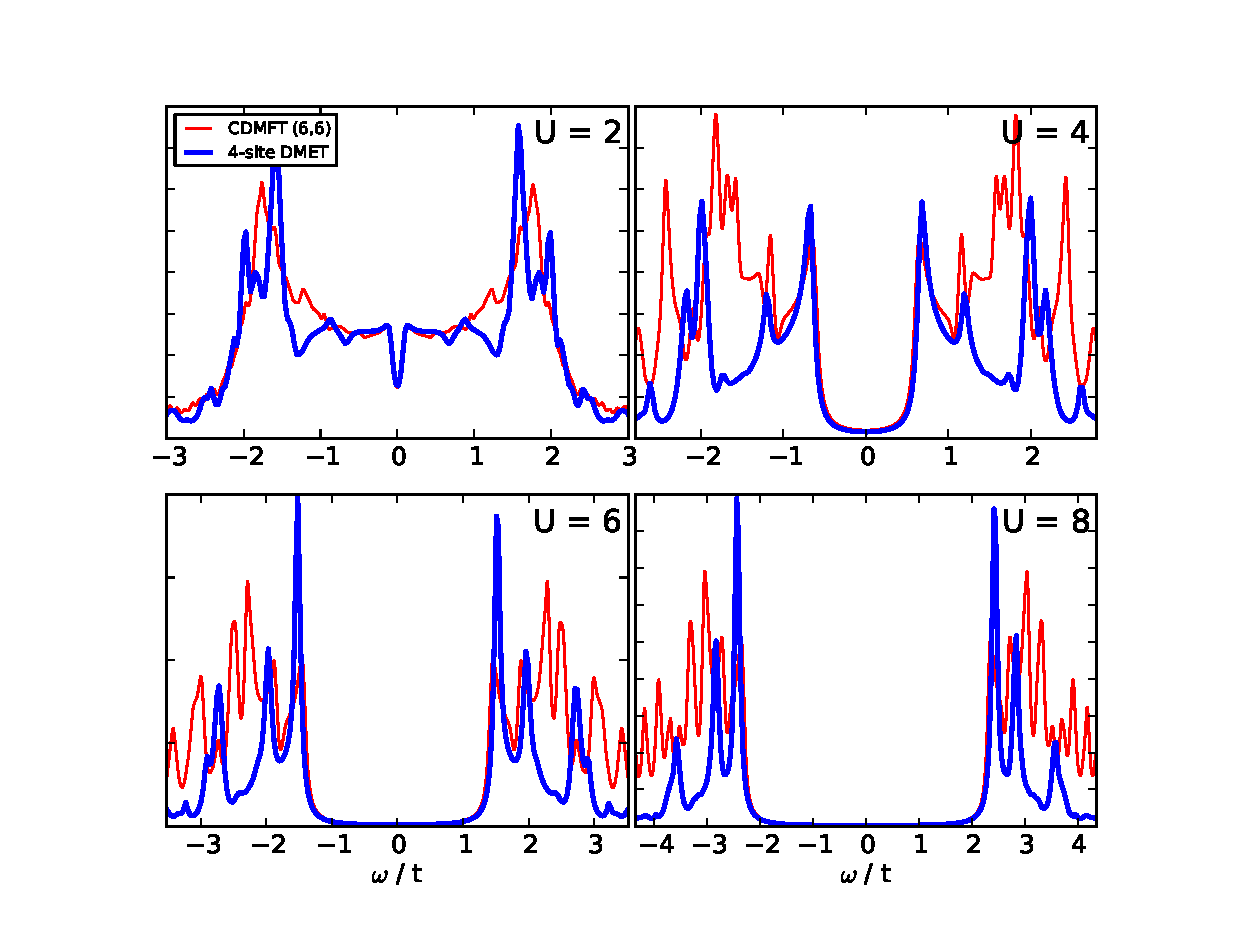
\includegraphics[scale=0.475]{Plots/1D_Spectra/1D_Hub_Spectra.eps}
\end{center}
\caption{Comparison of the local density of states from a four impurity cluster DMET calculation with a
(six impurity, six bath) CDMFT calculation for the half-filled 1D Hubbard model.}
\label{1D_DOS}
\end{figure}

%+++++++++++++++++++++++++++++++++++++++++++++++++++++++
%   1D HUBBARD SPECTRAL GAP 
%+++++++++++++++++++++++++++++++++++++++++++++++++++++++
\begin{figure}
\begin{center}
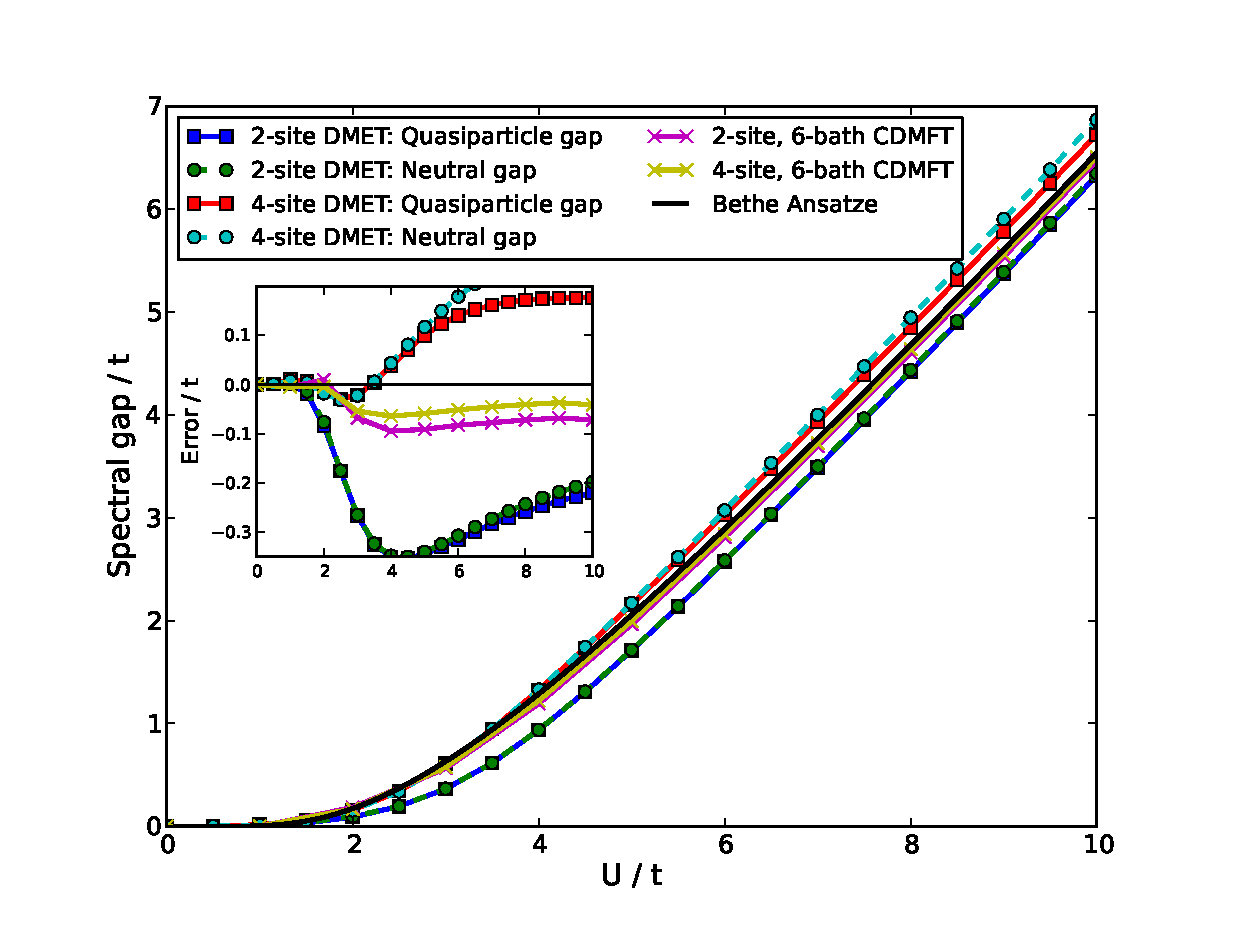
\includegraphics[scale=0.475]{Plots/1D_Gap/Hubbard_Gap.eps}
\end{center}
\caption{Spectral gap from the 1-particle and 2-particle greens functions compared to analytic results
from the Bethe Ansatze\cite{Ovchinni1970}.}
\label{1D_GAP}
\end{figure}


%+++++++++++++++++++++++++++++++++++++++++++++++++++++++
%   2D HUBBARD PLOTS 
%+++++++++++++++++++++++++++++++++++++++++++++++++++++++
\begin{figure}
\begin{center}
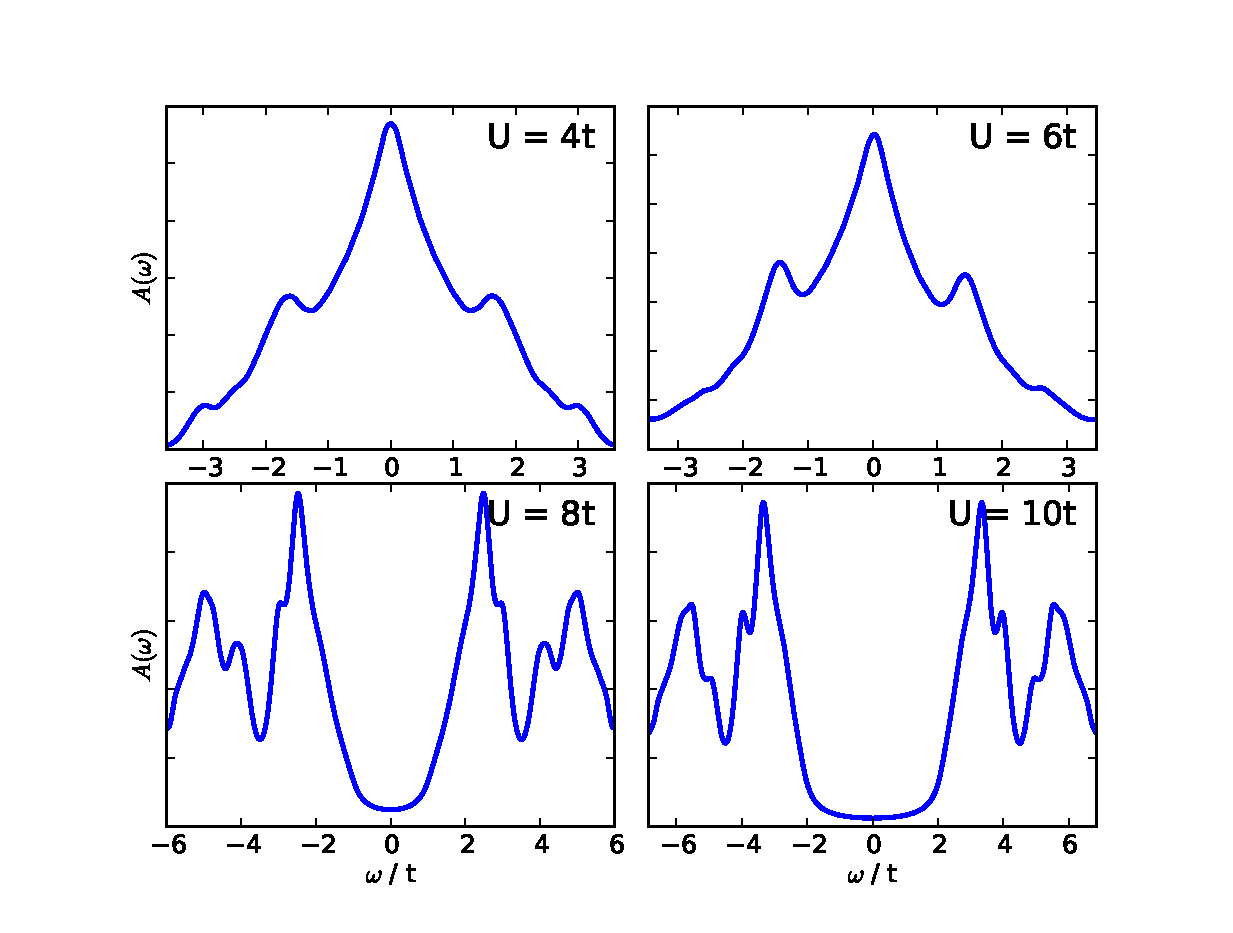
\includegraphics[scale=0.475]{Plots/2D_Spectra/2DHub_Spectra.eps}
\end{center}
\caption{Local density of states of the half-filled 2D hubbard model from a four impurity DMET calculation.}
\label{2D_DOS}
\end{figure}


%+++++++++++++++++++++++++++++++++++++++++++++++++++++++
%   2D DOPED HUBBARD PLOTS 
%+++++++++++++++++++++++++++++++++++++++++++++++++++++++
\begin{figure}
\begin{center}
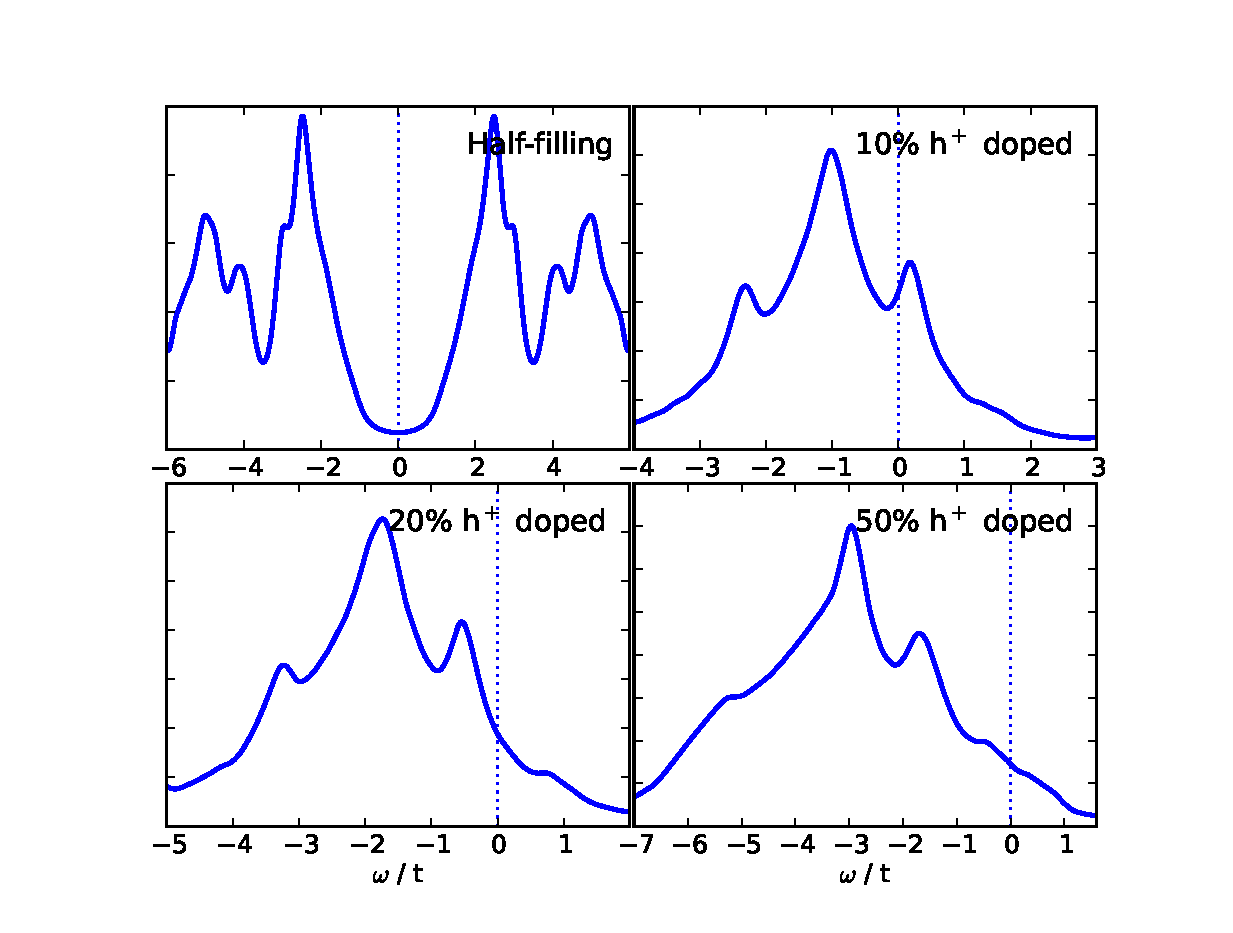
\includegraphics[scale=0.475]{Plots/Doping/2D/nImp4/U8/LargerBroadening/2DHub_Doping.eps}
\end{center}
\caption{Local density of states of the hole doped 2D hubbard model from a four impurity DMET calculation with $U = 8t$.}
\label{2D_Doped}
\end{figure}

%+++++++++++++++++++++++++++++++++++++++++++++++++++++++
%   DD response 
%+++++++++++++++++++++++++++++++++++++++++++++++++++++++
\begin{figure}
\begin{center}
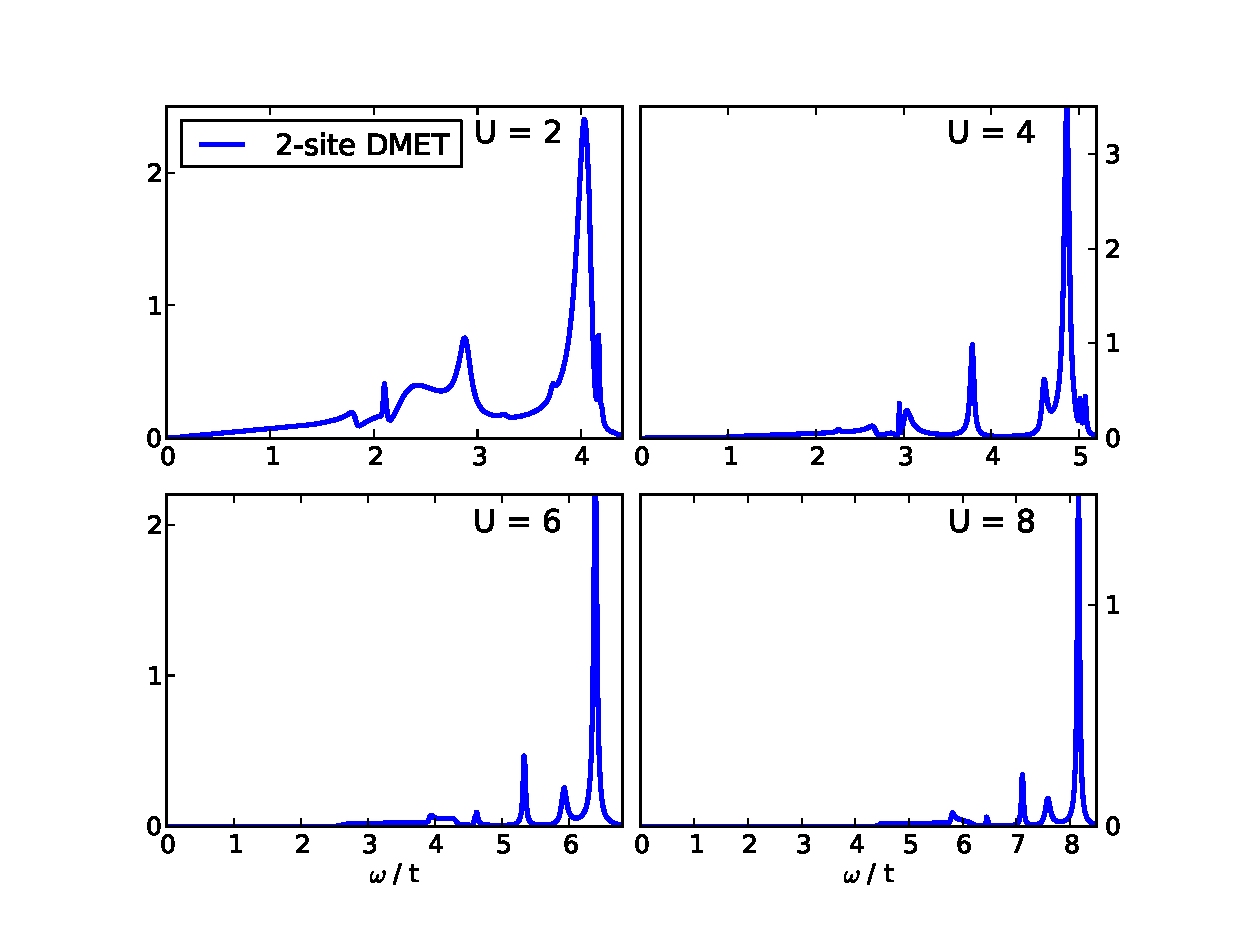
\includegraphics[scale=0.475]{Plots/1D_DD/1D_Hub_DD.eps}
\end{center}
\caption{Two impurity DMET calculation of the local density-density response function for the half-filled 1D hubbard model via construction of the 2-particle greens function.
The spectral gap is used in the data plotted in Fig.~\ref{1D_GAP}}
\label{1D_DD}
\end{figure}


TODO
----

Change 'ext' to some representation of the core orbitals.


\bibliography{SpectralDMETBib}

\end{document}
